\hfill \break
\justifying
Inicialmente fue considerada una Metodología de Prototipos, que cuenta con características similares a la metodología final escogida, difieriendo fundamentalmente en la filosofía de un desarrollo acelerado que pueda ofrecer una visión previa del producto, requiriendo una costante integración con el fin de realizar pruebas con los clientes e ir realizando las modificaciones o ajustes necesarios para cumplir con los requisitos dispuestos. Este enfoque aunque práctico, puede facilmente caer en el error de perder de vista los compromisos de calidad y mantenimiento que se acordaron con el cliente, derivado de las pruebas continuas presentadas al cliente rigiendo finalmente el desarrollo por una técnica basada en la prueba y el error.

\hfill \break
\justifying
Se ha decantado el desarrollo del proyecto por una Metodología basada en Componentes, por la naturaleza modular de la solución y los diferentes nodos y componentes que pueden irse mejorando independiente a la conformación completa del producto. Importante mencionar que el desarrollo independiente de cada componente requiere una definición correcta de los medios de conexión y protocolos de comunicación, facilitando y promoviendo una exitosa integración de todos los componentes.

\hfill \break
\justifying
Este paradigma considera un progreso de forma evolutiva adoptando muchas de las bondades que aporta un modelo en espiral, siendo una de las herramientas más beneficiosas y también las más problemáticas si no se aplican de forma correcta, el análisis de riesgos. La eficiente predicción de riesgos requiere de experiencia y habilidad derivada del conocimiento profundo de la problemática y la solución por aplicarse, lo que requirirá asesoría con especialistas en las tecnologías que se utilizarán y permitiendo disminuír la incertidumbre de la detección errada de los riesgos.

\hfill \break
\justifying
Entre los beneficios de la implementación de esta metodología se encuentra la simplificación de pruebas, pues estas son ejecutadas para cada uno de los componenetes antes de ser ensamblados en el conjunto. A su vez esto simplifica el mantenimiento general del sistema, así como su escala y propicia la calidad del sistema completo mejorando continuamente los componentes de forma independiente.

\hfill \break
\justifying
Finalmente resaltar la ventaja que aporta su cualidad incremental respecto a la búsqueda del modelo de aprendizaje automático, asegurando aquel con la mejor precisión de predicción y eficiencia en el desempeño durante su entrenamiento y finalmente la clasificación implementado directamente ya en el sistema embebido.


\begin{figure}[!h]
	\centering
	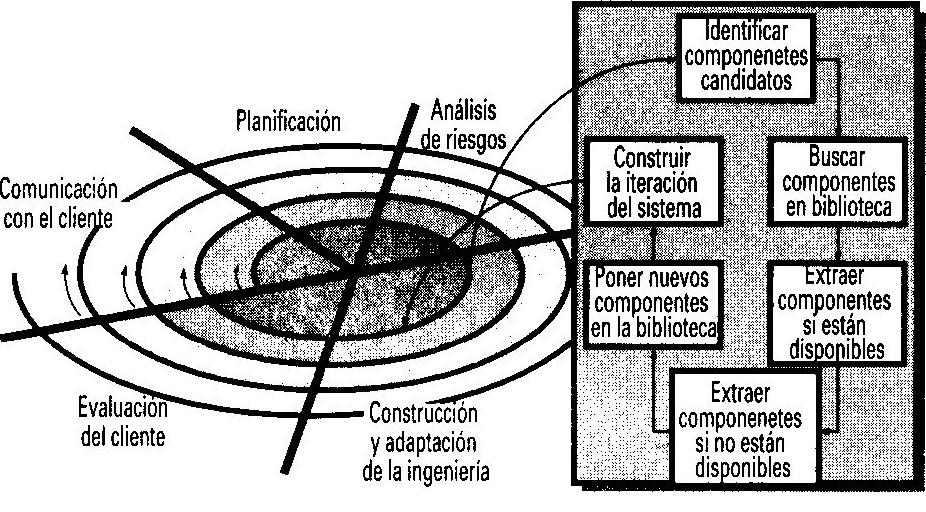
\includegraphics[width=14cm]{Imagenes/Modelo_componentes.jpeg}
	\caption{Diagrama mostrando el flujo iterativo y evolutivo de las etapas consideradas por la Metodología basada en el desarrollo por Componentes}
	\label{Metodologia_componentes}
\end{figure}